\documentclass{beamer} 
\usetheme{Hannover}
\usepackage{amsmath}
\usepackage{amsfonts}
\usepackage{amssymb}
\usepackage{graphicx}
\usepackage{wasysym}
\usepackage{comment}

\newcommand{\eps}{\varepsilon}
\newcommand{\inner}[1]{\left\langle #1 \right\rangle}
\newcommand{\abs}[1]{\left| #1 \right|}
\newcommand{\norm}[1]{\left\| #1 \right\|}
\newcommand{\wt}{\widetilde}
\newcommand{\tbf}{\textbf}
\newcommand{\R}{\mathbb{R}}
\newcommand{\C}{\mathbb{C}}
\newcommand{\Q}{\mathbb{Q}}
\newcommand{\Z}{\mathbb{Z}}
\newcommand{\N}{\mathbb{N}}
\renewcommand{\P}{\mathbb{P}}
\newcommand{\E}{\mathbb{E}}

\title{From Calculus to Machine Learning} 
\author{Paul Siegel}

\begin{document} 
\frame{\titlepage}

\frame{
What do linear regression, maximum likelihood estimation, support vector machines, and neural networks have in common?
\bigskip \pause

All fit into the following framework: \pause
\begin{itemize}
    \item Identify a space of ``reasonable'' models \pause
    \item Construct a function which computes how well a given model fits the data \pause
    \item Find the model(s) which maximize (or minimize) the function
\end{itemize}
}

\frame{
Data scientists play a significant role in this process: \pause
\begin{itemize}
    \item Identifying reasonable models uses domain expertise \pause
    \item Constructing a good objective function usually uses statistics \pause
    \item Finding the extremal model(s) uses math and/or engineering \pause
\end{itemize}

\bigskip

In this seminar we'll try to understand some of the theory behind all three steps.
}

\frame{
The plan:
\begin{enumerate}
    \item Optimization for functions of one variable
    \item Linear algebra and PCA
    \item Optimization for functions of several variables
    \item Conditional probability and Bayesian statistics
    \item Linear regression
    \item Perceptrons
    \item Back propagation and gradient descent
\end{enumerate}
}

\frame{
\frametitle{Optimizing quadratic functions of one variable}
You wish to build a rectangular fence next to a river.
You have 100m of fence to work with and you want to enclose as much area as possible.
How do you do it?
}

\frame{
What is the space of models?
\bigskip \pause

\begin{itemize}
    \item Each possible fence is determined by its height $x$ and its width $y$ \pause
    \item Constraints: $x \geq 0$, $y \geq 0$, and $2x + y = 100$
\end{itemize}
}

\frame{
What is the objective function?
\bigskip \pause

We want to maximize the area $A(x,y) = xy$
}

\frame{
This is now just a math problem: maximize $A(x,y) = xy$ subject to the constraints $x \geq 0$, $y \geq 0$, and $2x + y = 100$
\bigskip \pause

This is an example of a \textit{constrained optimization} problem.
\bigskip \pause

The objective function is quadratic and the constraint is linear, so we can hope to solve it analytically.
}

\frame{
Using the constraint, eliminate $y$ to get:

$$A(x) = x(100 - 2x)$$ \pause

\begin{center}
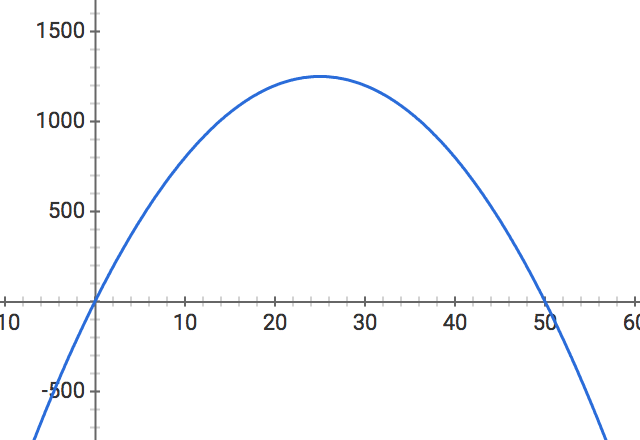
\includegraphics[scale = .5]{images/fence_graph.png}
\end{center}
}

\frame{
Algebraic magic:

$$A(x) = x(100 - 2x) = -2(x - 25)^2 + 1250$$ \pause

Since 

$$-2(x - 25)^2 \leq 0$$ \pause

we get

$$A(x) \leq 1250$$

with equality if and only if $x = 25$
}

\frame{
How does the algebraic magic work? \pause
\bigskip

Start with an expression of the form $x^2 + bx$. \pause

\begin{center}
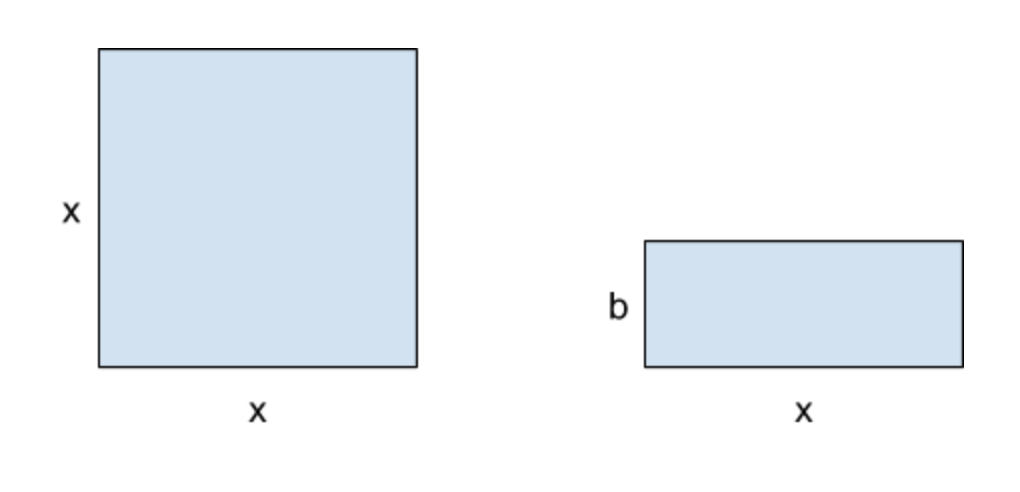
\includegraphics[scale = .5]{images/complete_square1.png}
\end{center}
}

\frame{
Cut the $bx$ rectangle in half and rearrange: \pause

\begin{center}
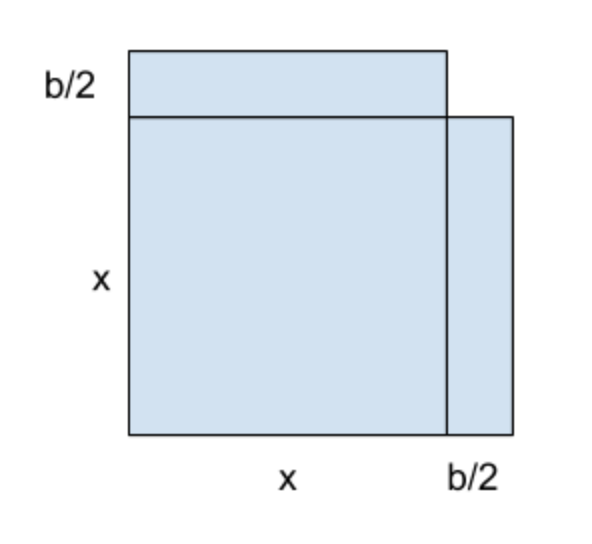
\includegraphics[scale = .5]{images/complete_square2.png}
\end{center}
}

\frame{
Complete the square! \pause

\begin{center}
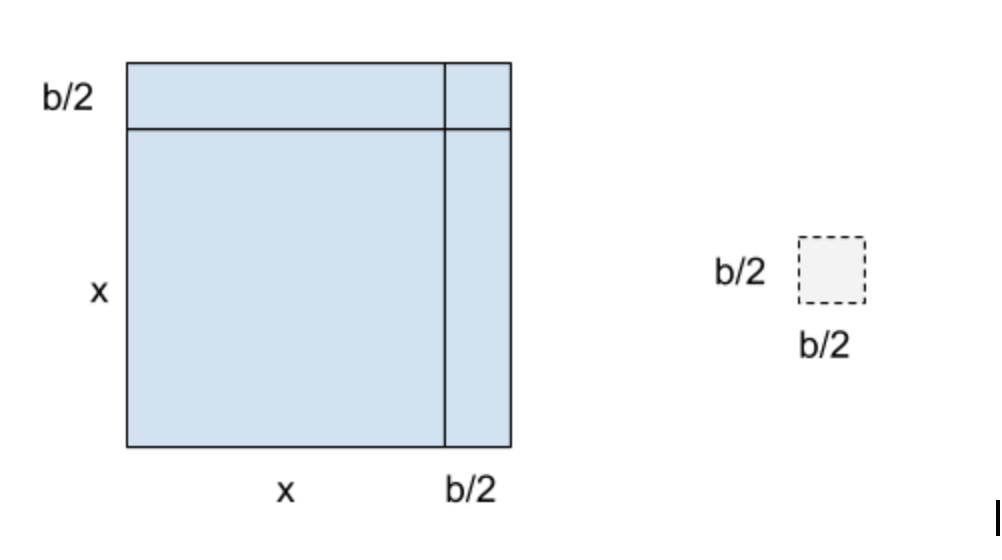
\includegraphics[scale = .5]{images/complete_square3.png} \pause
\end{center}

Conclusion:

$$x^2 + bx = \left( x + \frac{b}{2} \right)^2 - \frac{b^2}{4}$$
}

\frame{
In the example above, it looks like this: \pause

\begin{align*}
    A(x) &= x(100 - 2x) \\
         &= -2x^2 + 100x \\
         &= -2(x^2 - 50x) \\
         &= -2((x-25)^2 - 625) \quad \text{magic!} \\
         &= -2(x - 25)^2 + 1250
\end{align*}
}

\frame{
You want to build an open box with a square base which holds $25m^3$ of water.  How much material do you need?
}

\frame{
Space of models: \pause

\begin{\itemize}
    \item Each box is determined by the width $x$ of the base and the height $y$ \pause
    \item Constraints: $x \geq 0$, $y \geq 0$, $\text{Volume} = x^2y = 25$
\end{itemize}
}

\frame{
Objective function: \pause

\bigskip

We want to minimize the surface area $S(x,y) = x^2 + 4xy$
}

\frame{
Constrained optimization problem: minimize $S(x,y) = x^2 + 4xy$ subject to the constraints $x \geq 0$, $y \geq 0$, and $x^2 y = 25$. \pause

\bigskip

The objective function is quadratic, but the constraint $x^2 y = 25$ is cubic, so we expect this to be harder.
}

\frame{
Use the constraint to eliminate $y$ and get: \pause

$$S(x) = x^2 + \frac{100}{x}$$ \pause

\begin{center}
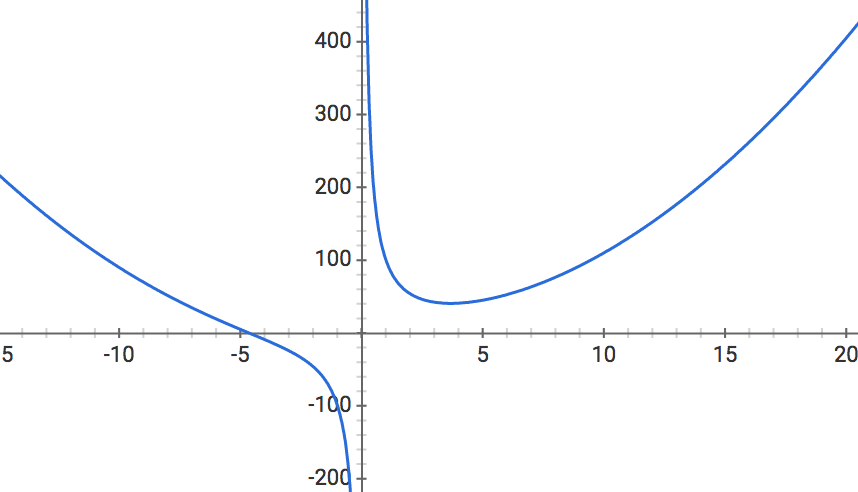
\includegraphics[scale = .5]{images/open_box_graph.png}
\end{center}
}

\frame{
No algebraic magic; we'll need some tools. \pause

\bigskip

Main idea: approximate a general function with a quadratic function.
}

\end{document}
